This thesis investigates stellar streams originating from globular clusters in the Milky Way. Stellar streams are long, thin structures composed of stars that have escaped their host stellar system, forming coherent tails that can span large regions of the sky (Fig.~\ref{fig:S5MilkywayStreams}). Globular clusters were first systematically cataloged by Charles Messier in the late 1700s--not for their scientific interest at the time, but to help comet hunters avoid mistaking these nebula-like objects for new comets \citep{1781cote.rept..227M}. Many of the most prominent globular clusters, along with diffuse nebulae and external galaxies, are included in the Messier catalog (Fig.~\ref{fig:All_messier_objects}). Physically, globular clusters are dense, gravitationally bound systems containing hundreds of thousands to millions of stars, and are an important source of stellar streams.
\begin{figure}
    \centering
    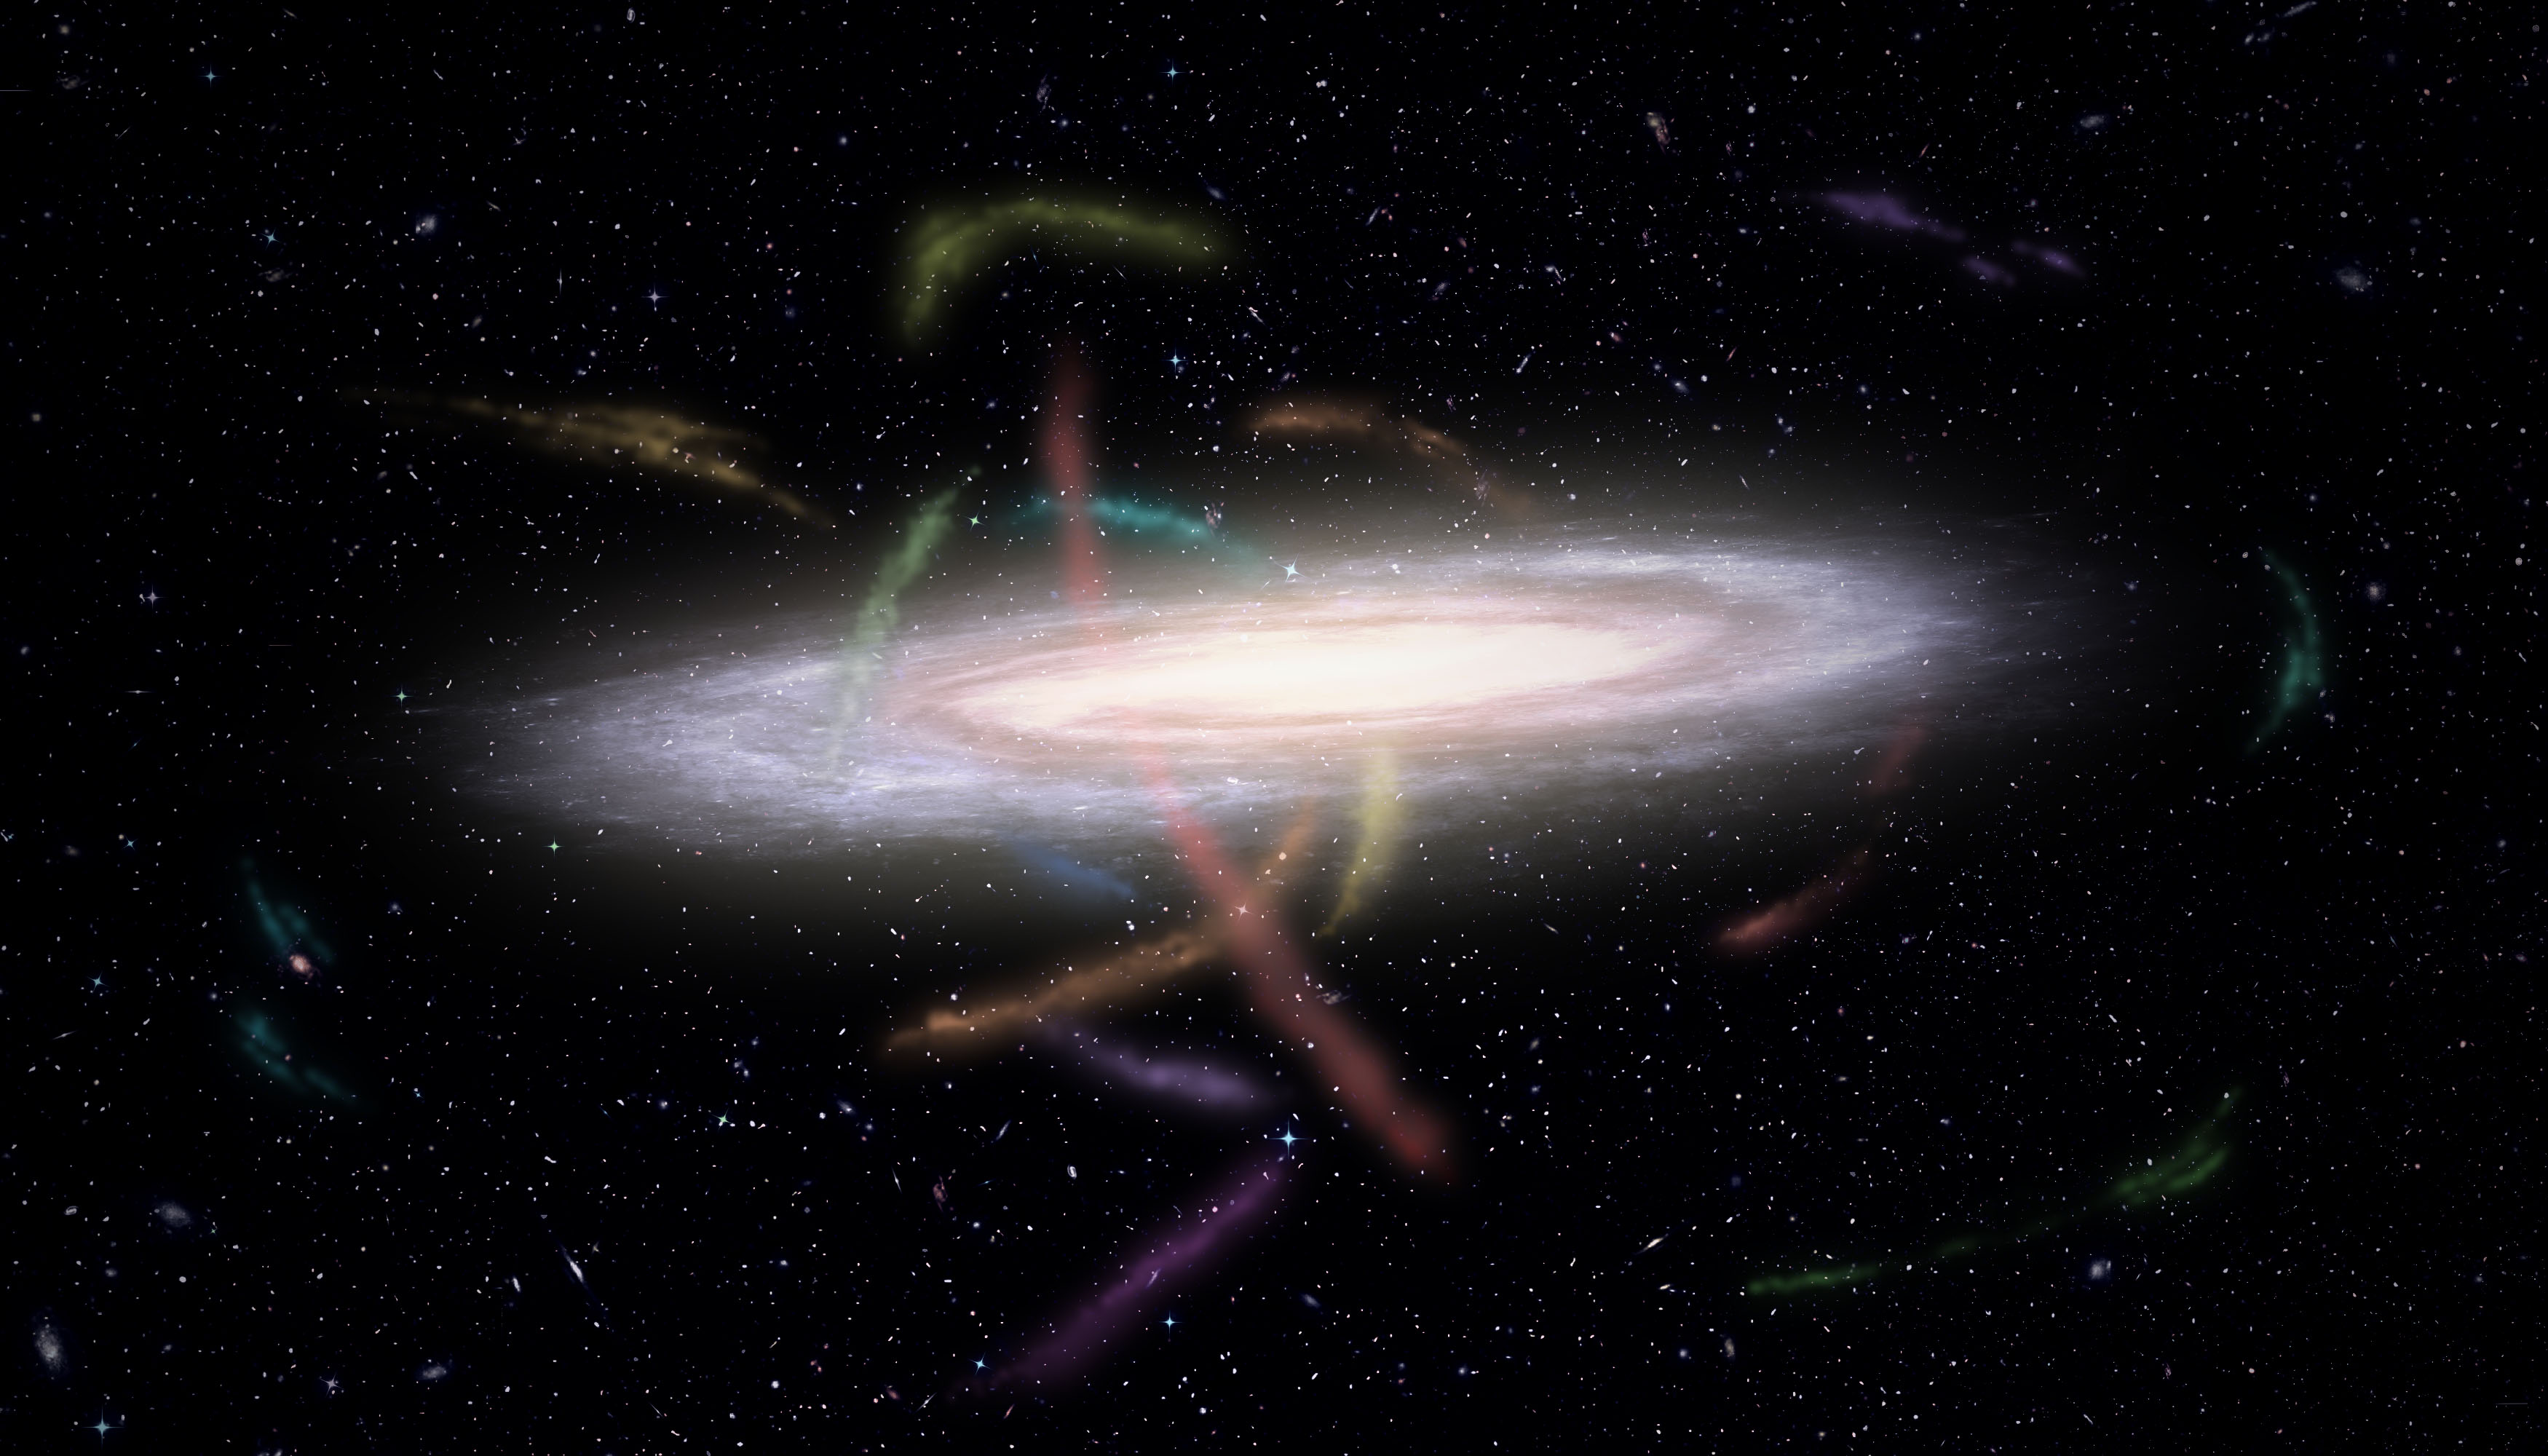
\includegraphics[width=\linewidth]{images/S5MilkywayStreams.jpg}
    \caption[Artist Rendition of Stellar Streams]{An artist's rendition of a galaxy surrounded by stellar streams. Credit: James Josephides and S$^5$ Collaboration \citep{2019MNRAS.490.3508L}.}
    \label{fig:S5MilkywayStreams}
\end{figure}

In Chapter 4, I present our study in which we simulated the expected distribution of stellar streams originating from the entire Milky Way globular cluster system. This study was the first of its kind. Stellar streams have high hopes for being inferential tools for fine details of the gravitational field of the Milky Way, notably for constraining the presence of \textit{dark mater subhalos}. These halos may perturb the stellar streams leaving ``gaps'' in their wake. Since structure of stellar streams are sensitive to local and global gravitational field, all phenomena that can influence the streams must be well calibrated to ensure proper inference of the distribution of dark matter within the Milky Way. In Chapter~5, we explored how the collective gravitational influence of all globular clusters can perturb streams to produce such gaps.

\begin{figure}
    \centering
    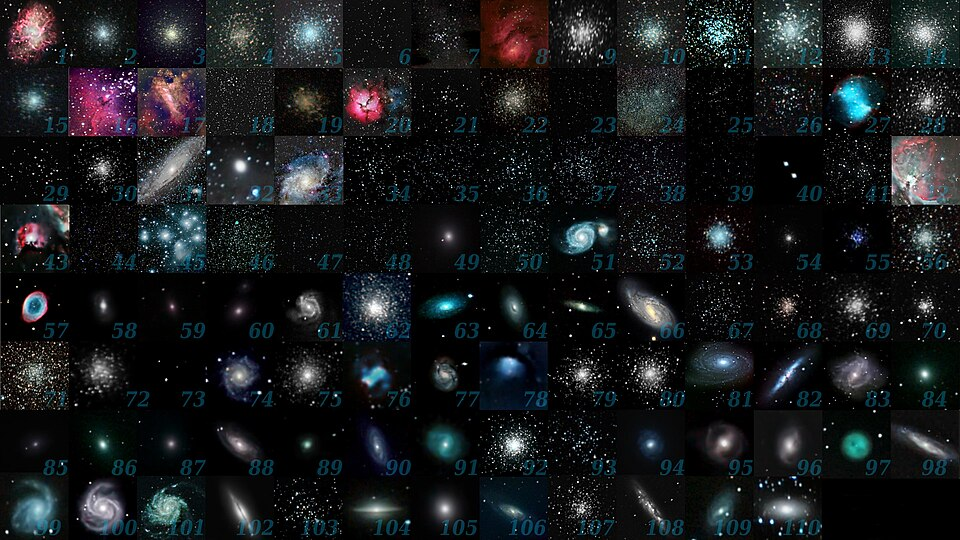
\includegraphics[width=\linewidth]{images/All_messier_objects.jpg}
    \caption[Messer objects]{The Messier catalog containing ``nebulae-like'' objects: planetary nebulae, diffuse nebulae, supernovae remenants, open clusters, globular clusters, and foreign galaxies. By Michael A. Phillips, an amateur astronomer. - http://astromaphilli14.blogspot.com.br/p/m.html official blog, CC BY 4.0, https://commons.wikimedia.org/w/index.php?curid=38121043}
    \label{fig:All_messier_objects}
\end{figure}

The structure of the thesis is as follows. The remainder of the introduction provides background on stellar streams, globular clusters, and their astrophysical context, as well as an overview of the current state of the field. Chapter~2 outlines the physical framework used to model stream formation and interpret their morphology. Chapter~3 describes the numerical methods employed in the simulations, including convergence tests and estimates of computational cost. Chapters~4 and~5 present two published studies, with the final chapter discussing these results in the broader context of the literature and highlighting future directions.

\section{General context}
    Before explaining why Milky Way globular clusters and stellar streams are scientifically interesting, it is important to first set the scene. This thesis fits neatly within the field of galactic astronomy, which, at its core, studies the current state of our galaxy and the processes that shaped its formation within the broader context of the universe.

    If we start this narrative from the beginning and place stellar streams and globular clusters in the timeline of cosmic history, their importance becomes clear. The story begins best at the very start. The Lambda Cold Dark Matter ($\Lambda$CDM) cosmological model is currently the leading theory of the universe, successfully unifying a variety of observational evidence from the Cosmic Microwave Background Radiation and the large-scale distribution of galaxies to the accelerating expansion of the universe, etc. \citep{2001LRR.....4....1C,2022NewAR..9501659P}.

    Shortly after the Big Bang, conditions allowed protons, neutrons, and electrons to form and interact. For a few minutes, these particles collided and fused into heavier elements in a process known as Big Bang Nucleosynthesis \citep{2007ARNPS..57..463S}. When this phase ended, the universe's composition was mostly hydrogen, deuterium ($^2$H), helium-4 ($^4$He), and trace amounts of helium-3 ($^3$He) and lithium-7 ($^7$Li). By mass, hydrogen made up roughly 75\%, and helium about 25\% of the primordial universe \citep{1966ApJ...146..542P,2016RvMP...88a5004C}.

    $\Lambda$CDM positis the existence of Dark matter and that it has about five times more mass than ordinary matter \citep{2020A&A...641A...6P}. Dark plays a critical role in galaxy formation. In the early universe, dark matter was distributed nearly uniformly. Over dense regions caused it to collapse into a cosmic web of filaments and nodes. These massive nodes created deep gravitational wells that attracted ordinary matter \citep{1974ApJ...187..425P}. The infalling gas subsequently cooled and formed stars. The resulting complex of stars, gas, and dark matter constitutes a galaxy \citep{2008LNP...740.....P,2010gfe..book.....M}.

    Galaxies contain stars that are born, fuse hydrogen and helium into heavier elements, and eventually die, often as supernovae, enriching the interstellar medium with these heavier elements \citep{2019A&ARv..27....3M}. The stellar formation process is a strong function of cosmic time as the chemical evolution of the universe becomes more metal rich. For example, the first generation of stars, known as Population III (Pop III) stars\footnote{Stellar populations are named in reverse order of discovery. Population I stars are the youngest, metal-rich stars (including the Sun), Population II stars are older and metal-poor, and Population III stars are the very first, metal-free stars.}, formed in a very different environment, one devoid of metals \citep{2002Sci...295...93A,2005SSRv..117..445G,2013RPPh...76k2901B}. 

    The chemical composition of the gas is crucial since it influences the initial mass function (IMF) of stars. Stars formed from pristine, metal-free gas tend to have a top-heavy IMF, favoring the formation of massive stars \citep{2002ApJ...571...30S,2006MNRAS.369..825S}. In contrast, even small amounts of metals introduced into the gas can dramatically shift the IMF toward the favoring the formation of lighter stars \citep{2021MNRAS.508.4175C}.

    Globular clusters are, to first approximation, single-stellar populations: their constituent stars formed from the same molecular cloud over a timescale shorter than the internal dynamical time \citep{1988ApJ...324..288A,2009MNRAS.397..954F,2014PhR...539...49K}. Owing to their uniform chemical composition, stellar evolution within a cluster proceeds along the color-magnitude diagram as a function solely of initial mass \citep{2013sse..book.....K}. This property enables precise age determinations from photometric observations, a method that historically provided the first robust lower limits on the age of the Universe \citep{1959MNRAS.119..124H,1970ApJ...162..841S,1985A&A...147..169G,1992ApJ...400..265M}. With their low metallicities and advanced ages, globular clusters are dominated by Population~II stars, indicating that they formed in environments enriched exclusively by the earliest generations of stars \citep{2022A&A...668A.191C}. They thus constitute valuable fossil records of the initial phases of star formation and chemical evolution in the Universe.
    
    Globular clusters are among the most ubiquitous stellar systems in the Universe \citep{2006ARA&A..44..193B,2019ARA&A..57..227K}. They are found in virtually all galaxy types, from dwarfs to giant ellipticals, and their total number correlates with global properties of their host galaxies such as mass and luminosity \citep[e.g.,][]{2013ApJ...772...82H,2018MNRAS.481.5592F}. In the local Universe, we can directly observe the formation of massive bound stellar systems—so-called young massive star clusters—which may represent present-day analogs of the GC formation process \citep[e.g.,][]{2010ARA&A..48..431P,2020SSRv..216...69A}, though whether all such systems will evolve into globular clusters remains an open question.

    Globular clusters serve as unique astrophysical laboratories, offering insights into stellar dynamics, stellar evolution, and galaxy assembly. Their evolution involves stellar structure and evolution, gravitational dynamics, and relativistic effects in dense environments. For instance, close stellar encounters and binary interactions—such as mass transfer or mergers—are common in such environments and significantly shape cluster evolution \citep{2004MNRAS.349..129D,2016MNRAS.458.1450W,2024MNRAS.528.5119A}. Additionally, globular clusters are suspected to be a pathway for forming intermediate-mass black holes (IMBHs) \citep{2013MNRAS.432.2779B,2015MNRAS.454.3150G}. The origin of IMBHs remains uncertain, as their masses are too large to be explained by isolated stellar evolution, yet too small to fall into the supermassive category \citep{2020ARA&A..58..257G}. 
    
    Moreover, while traditionally considered as single stellar population that are homogeneous in age and chemical composition, decades of spectroscopic and photometric evidence have revealed the presence of multiple stellar populations in most GCs \citep{2008MNRAS.391..825D,2011ApJ...726...36C,2012A&ARv..20...50G,2018ARA&A..56...83B}. The origin of these multiple populations remains debated, with proposed explanations ranging from self-enrichment to accretion of external material, but no consensus has yet emerged.

    % \citet{2025arXiv250116438K} proposes that the main formation of globular cluster formation is at high redshift galaxies in high pressure environments. However, other mechanisms can exist as well and contribute to this.
    
    % \citet{2018RSPSA.47470616F} also discusses two different formation scenarios. That GCs form naturally at high redshift. Or that they form within dark matter sub halos. 
    
    % \citep{2016ApJ...823...52K} talks about  the formation of globular clusters within dark matter sub-halos. it's awesome! they discuss prestine gas and also evoke enrichment from pop III and pop II stars. They ran some hydro dynamical simultions. 

    A striking property of many GC systems is the bimodality in their metallicity distribution, with one population of metal-poor GCs and another of metal-rich GCs \citep[e.g.,][]{2006ARA&A..44..193B, 2015ApJ...806...36H}. This bimodality is now widely interpreted as evidence for multiple formation channels: metal-rich GCs likely formed in situ within the main progenitor galaxy during intense star-formation episodes, whereas metal-poor GCs were predominantly accreted from lower-mass satellites. The persistence of this bimodality across a wide range of galaxies suggests that hierarchical accretion has been a fundamental process shaping GC systems.

    From the perspective of galaxy formation, the hierarchical model of structure growth posits that galaxies assemble through repeated mergers and accretion of smaller systems \citep{2015ARA&A..53...51S}. In this framework, GCs can form in situ within the main progenitor or be accreted from satellite galaxies \citep[e.g.,][]{2018MNRAS.479.4760F,2020MNRAS.498.2472K,2021ApJ...920...51M,2022ApJ...930L...9M,2023A&A...673A..86P,2024MNRAS.528.3198B,2025A&A...693A.155P}. Consequently, the spatial distribution, kinematics, chemical abundances, and metallicity substructure of a galaxy's GC system retain valuable information about its merger history and assembly pathways. This makes GCs not only tracers of early star formation, but also fossil records of the build-up of their host galaxies.

    In essence, globular clusters are involved in many astrophysical processes such as the hierarchical formation of galaxies, formation of intermediate black holes, and being products of barely enriched gas in the early states of the universe \citep{2016ApJ...823...52K,2025arXiv250116438K}. Fully understanding their formation and evolution ties neatly into a variety of astrophysical problems.

    Globular clusters are of considerable astrophysical interest—not only for studies of stellar formation and evolution, rich internal dynamics, black hole formation, and their role in the build-up of galaxies—but also because they are prolific progenitors of \textit{stellar streams}. As we will show in the next chapter, tidal forces excite stars within the clusters to eventually escape with small speeds that keep the ejected material along more or less the same trajectory, creating the stellar streams.

    These streams are particularly valuable astrophysical tools. Their discovery and theoretical explanation date back to the 1990s (see the introductions to Chapters~4 and~5), after which both observational and theoretical work accelerated rapidly. For example, \citet{2002MNRAS.332..915I} proposed that stellar streams could be sensitive probes of the dark matter subhalo population (see Chapter~5 for a more detailed discussion).

    Because stellar streams trace extended, coherent arcs across the sky, they serve as natural guides for mapping the Galactic gravitational field. \citet{2010ApJ...712..260K} used the GD-1 stream to constrain the Milky Way potential, while \citet{2011MNRAS.417..198V} performed numerical experiments demonstrating that streams can constrain their host potential even with incomplete phase-space information (e.g., sky positions alone, positions plus radial velocities, or positions plus distances). \citet{2016ApJ...833...31B} also applied this approach to the Palomar~5 and GD-1 streams, and \citet{2010ApJ...718.1128L} investigated the shape of the Galactic dark matter halo using the Sagittarius stream.

    These pioneering studies demonstrated the potential of stellar streams as astrophysical probes, but they represented only the beginning. With the advent of the \emph{Gaia} mission, the volume and precision of available data have transformed what is possible.

\section{The state of the art}
    The current era of Galactic astronomy is undoubtedly defined by the \emph{Gaia} space mission \citep{2016A&A...595A...1G,2016A&A...595A...2G,2018A&A...616A...1G,2021A&A...650C...3G,2023A&A...674A...1G}. The European Space Agency's space-based observatory has been conducting continuous observations of the sky to perform precise astrometric measurements. Operating since 2014, Gaia improves its data volume and quality each year through repeated parallax measurements.  As of Data Release~3, the mission has provided distances and proper motions for nearly two billion stars in the Galaxy, along with millions of radial velocity measurements \citep{2023A&A...674A...1G}. This yields five-dimensional phase-space information (positions and on-sky velocities) for about 1-2\% of the Galactic stellar population. Although the radial velocities are limited to relatively bright stars, the resulting dataset is still unprecedented in scope.

    When additional measurements are required, \emph{Gaia} data are often complemented with observations from other facilities.  For example, \emph{Gaia} struggles to determine parallaxes in the crowded interiors of globular clusters, where high stellar densities pose challenges for its instruments \citep{2017MNRAS.467..412P}. To address this, \citet{2021MNRAS.505.5957B} combined \emph{Gaia}~EDR3 astrometry with \emph{Hubble Space Telescope} observations, enabling precise distance measurements for 162 globular clusters.

    Several ground-based spectroscopic surveys aid in extending \emph{Gaia}'s radial velocity measurements to fainter magnitudes. Examples include the Apache Point Observatory Galactic Evolution Experiment (APOGEE; \citep{2017AJ....154...94M}), the Gaia-ESO Survey \citep{2023A&A...676A.129H}, and upcoming wide-field facilities such as 4MOST \citep{2019Msngr.175....3D} and WEAVE \citep{2014SPIE.9147E..0LD}.  Other large surveys primarily focus on providing detailed chemical abundances for a wide range of stellar populations, including GALAH \citep{2012ASPC..458..421Z}, the Gaia-ESO Survey \citep{2023A&A...676A.129H}, PAN-STARRS \citep{2016arXiv161205560C}, and APOGEE \citep{2017AJ....154...94M}, often delivering both radial velocities and multi-element abundance measurements in the same observations.

    These large data sets have led to a rapidly increasing number of stellar stream discoveries. With the advent of the \texttt{streamfinder} algorithm \citep{2018MNRAS.477.4063M,2018MNRAS.478.3862M}, many streams could be detected simultaneously. This was possible because \texttt{streamfinder} agnostically applies a friend-finding algorithm to identify coherent stellar groups in the data. It was initially applied to a small number of streams to reassess their properties and discuss their characteristics in light of the improved quality and quantity of the data \citep{2019NatAs...3..667I,2020ApJ...891..161I}.

    Encouraged by these initial successes, the method was scaled up to the full \emph{Gaia} dataset, allowing for a systematic search across a much larger region of the sky. \citet{2021ApJ...914..123I} subsequently applied \texttt{streamfinder} to \emph{Gaia}~DR2 and EDR3, resulting in a major increase in the number of known stellar streams. This analysis improved the data quality for many previously known streams and led to several new detections, a selection of which is reproduced in Fig.~\ref{fig:ibata_2021_fig1}. They reported nine new streams, bringing the total number of known Galactic stellar streams to about sixty. 
    \begin{figure}
        \centering
        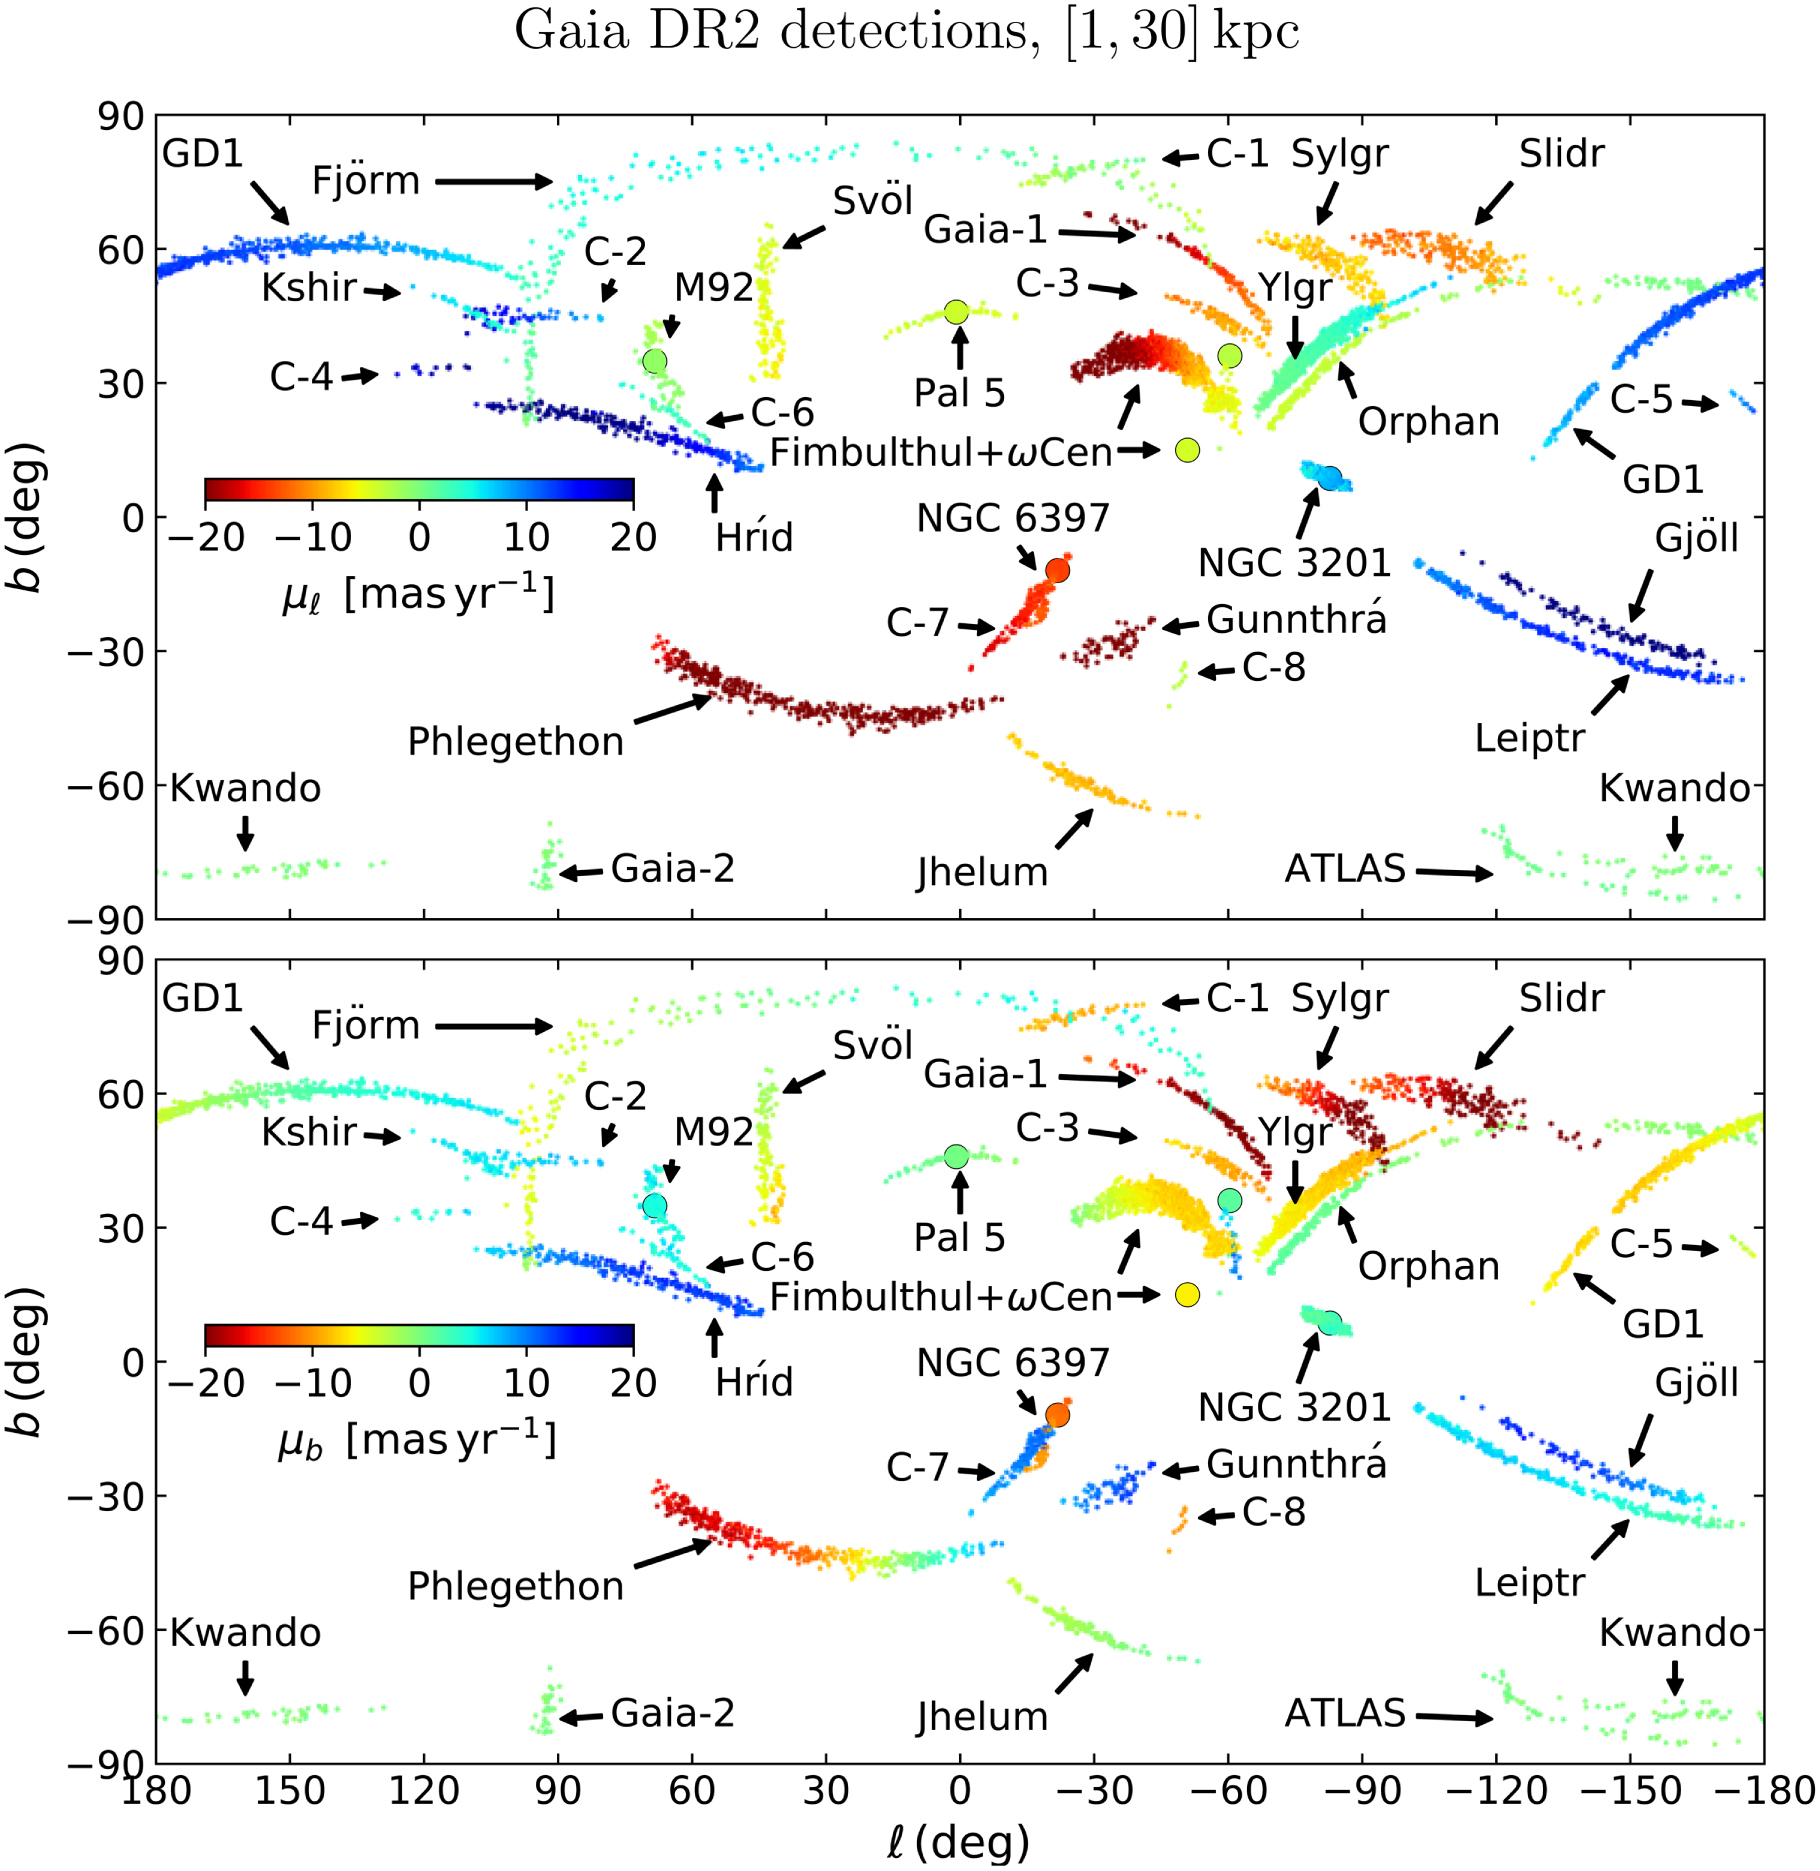
\includegraphics[width=\linewidth]{images/ibata_2021_fig1.jpg}
        \caption[Milky Way stellar streams discovered with \texttt{streamfinder} in \emph{Gaia} DR2]{Milky Way stellar streams discovered with \texttt{streamfinder} in \emph{Gaia}~DR2. Both plots are shown in Galactic coordinates. The top panel is color-coded by proper motion in longitude, while the bottom is color-coded by proper motion in latitude. This is Fig.~1 from \citet{2021ApJ...914..123I}.}
        \label{fig:ibata_2021_fig1}
    \end{figure}
    The work of \citet{2021ApJ...914..123I} was a primary motivation for this study. They showed that, of the roughly sixty stellar streams known at the time, only twenty were associated with globular clusters.  As summarized in \citet{2020A&A...637L...2P}, no clear correlations have been found between a cluster's orbital or structural parameters and the presence (or absence) of tidal tails. This motivated our simulation of the expected mass-loss distribution for the entire Milky Way globular cluster population, presented in Chapter~4.

    The improved quality and completeness of stellar stream catalogs in the Gaia era have rapidly expanded the scope of scientific applications. With these data, many studies have already begun to address a wide range of questions, including:  
    \begin{enumerate}
        \item reconstructing the accretion history of the Milky Way;
        \item measuring the local and global gravitational potential;
        \item probing the influence of time-dependent dynamical processes such as the bar, giant molecular clouds, and dark matter subhalos.
    \end{enumerate}
    A recent review by \citet{2025NewAR.10001713B} provides a comprehensive overview of some of these efforts. Usefully, they classify stream morphology as the result of three main factors: (1) the internal dynamics of the progenitor system, which determine the rate and energy of escaping stars; (2) the smooth, time-independent gravitational field, which sets the orbital path and tidal forces; and (3) time-dependent perturbations, including those from baryonic and dark matter substructure. We refer the reader to that review for a detailed discussion, and return to some of these aspects in Chapters~4 and~5.

    Stellar streams are also providing new insights into globular cluster formation. Several proposed scenarios exist, one of which suggests that clusters formed within their own dark matter subhalos \citep{2025arXiv250116438K}. While kinematic studies have explored the consequences of this hypothesis \citep{2022A&A...667A.112V}, current evidence disfavors it. For example, \citet{2016ApJ...823...52K} showed that clusters forming in deep dark matter potential wells would display metallicity spreads larger than those observed, and \citet{2022ApJ...941L..38M} used Gaia data to demonstrate that the velocity dispersions of several Milky Way streams are inconsistent with predictions for clusters embedded in massive, cuspy halos.

    Streams can also help distinguish between globular cluster and dwarf galaxy progenitors \citep{2021ApJ...909L..26B}. For instance, \citet{2020ApJ...898L..37Y} discovered a metal poor ``Low Mass Stream''  which they were able to associate dynamically with two globular clusters and argued that one of the clusters was actually the nuclear star cluster of the now defunk dwarf galaxy that has been completely merged into the Milky Way. \citet{2021ApJ...920...51M} further characterized the stream and remarked that it has a broad metallicity distribution and a high velocity dispersion—properties more consistent with a disrupted dwarf galaxy than with a globular cluster. 
    
    \citet{2022MNRAS.516.5331M} presented the metallicity of over 25 streams that were detected with \texttt{streamfinder} using the to PRISTINE survey \citep{2017MNRAS.471.2587S}. \citet{2022MNRAS.516.5331M} found that many streams are indeed metal poor. Despite the fact that globular clusters are already metal-poor objects compared to tyipcal field stars within the galactic disk \citep{\citet{2006ARA&A..44..193B}}, Peculiarly, some streams are even more metal poor than all the known globular clusters \citet{2020Natur.583..768W,2025A&A...698A..82Y}. \citet{2022MNRAS.516.5331M} suggested the stream maybe a fossil of a low-mass dwarft galaxy but nonetheless reflect a very ancient interstellar medium in which the stars were formed since there was so little iron enrichment. 
    
    Next, regarding the gravitational potential of the Milky Way, streams are being used to probe the granularity of the Milky Way's gravitational field. A striking example is the GD-1 stream: \citet{2019ApJ...880...38B} identified a gap in its density profile and modeled it as the result of a perturbation by a massive object. Follow-up work by \citet{2020ApJ...892L..37B} localized a potential dark matter subhalo whose orbit is consistent with having originated from the Sagittarius dwarf galaxy. Such cases illustrate how streams can simultaneously constrain the Milky Way's assembly history and the distribution of dark matter substructure.

    The information content of streams in constraining the Galactic potential has been quantified by \citet{2018ApJ...867..101B}, who showed that a single stream cannot simultaneously constrain all relevant parameters due to strong degeneracies. However, they also demonstrated that fitting multiple streams jointly can break these degeneracies—an approach realized by \citet{2024ApJ...967...89I}, who used Gaia DR3 to discover even more streams using \texttt{streamfinder} and then employed roughly 20 to create a best fit model of the Milky Way's gravitational field.

    In summary, stellar stream science is rapidly evolving. The expanding stream catalog—enabled by Gaia and complementary surveys—is unlocking new opportunities to probe globular cluster formation, the accretion history of the Milky Way, the nature of the Galactic gravitational potential, and the properties of dark matter itself. As the number and quality of identified streams continue to grow, so too will their impact on Galactic archaeology.
